\chapter{Correlation Structure}
\label{ap:Correlatation}
In the book Gaussian Markov Random Fields, Rue and Held show the correlation structure between the hyper-parameter $\mu$ and the latent field $\bm{x}$, which slows down convergence especially when using Gibbs samplers.
They consider the hierarchichal sturcture
\begin{align}
	\mu \sim \mathcal{N}(0,1)\\
	\bm{x}|\mu \sim \mathcal{N}(\mu\bm{1},\bm{Q}^{-1}) \, ,
\end{align}
and use a Gibbs sampler over the full conditionals
\begin{align}
	\mu^{(k)} | \bm{x}^{(k)} &\sim \mathcal{N} \Bigg(\frac{\bm{1}^T\bm{Q}\bm{x}^{(k-1)}}{1 + \bm{1}^T\bm{Q}\bm{1}}, (1 + \bm{1}^T\bm{Q}\bm{1})^{-1} \Bigg)\\
	\bm{x}^{(k)} | \mu^{(k)} &\sim \mathcal{N} (	\mu^{(k)}\bm{1}, \bm{Q}^{-1}) \, .
\end{align}
In Figure \ref{fig:RueHeld} one can clearly see that when steps only in the $\mu$-direction, x-axis, or in the $\bm{x}$-direction, vertical-(y)-axis, are allowed it takes a lot of steps to explore the parameter space due to high correlation in between $\mu$ and $\bm{x}$.
\begin{figure}[ht!]
	\centering
	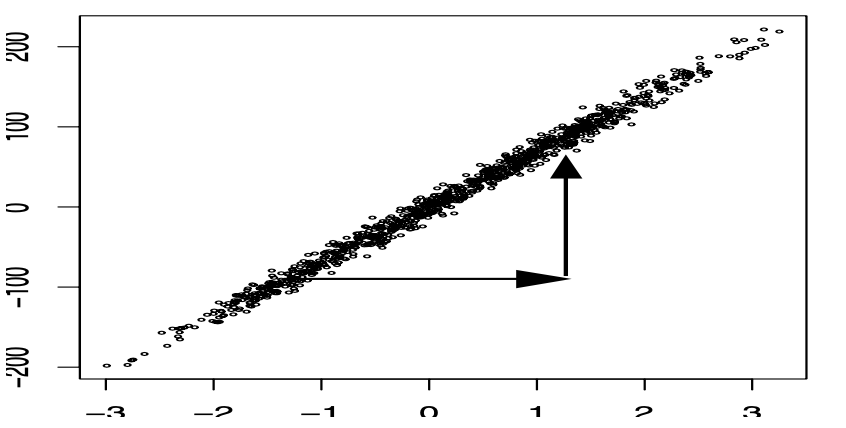
\includegraphics[width = \textwidth]{Figures/RueHeldBookFig.png}
	\caption[Correlation structur]{Figure 4.1 Figure (a) shows the marginal chain for µ over 1000 iterations of
		the marginal chain for the hyperparmeter with a specuifuc autoregressive proces defined in $\bm{Q}$ The algorithm
		updates successively $\mu$ and $x$ from their full conditionals. Figure (b) displays
		the pairs ($\mu(k)$ ,  $1^T\bm{Q}x(k)$ ), with$\mu(k)$ on the horizontal axis. The slow mixing
		(and convergence) of $\mu$is due to the strong dependence with $1^T\bm{Q}x(k)$  as only
		horizontal and vertical moves are allowed. The arrows illustrate how a joint
		update can improve the mixing (and convergence)}
	\label{fig:RueHeld}
\end{figure}
A solution is to update $(\mu, x)$ jointly, where, since $\mu$ is one dimensional, effectively only marginal density of $\mu$, by integrating out $\bm{x}$  of the joint density $\pi(\mu, x)$, is needed.
\begin{align}
	\mu^{\star}  &\sim q (\mu^{\star}|	\mu^{(k-1)} ) \\
	\bm{x}^{(k)} | \mu^{\star} &\sim \mathcal{N} (	\mu^{\star}\bm{1}, \bm{Q}^{-1}) 
\end{align}
With a simple MCMC algorithm on $ \mu$ one can explore the sample space of $\mu$ and only draw a sample $\bm{x}$ from its full conditional after e.g.  $\mu^{\star}$ is accepted. 



\chapter{Mesure theroy}
\label{ch:Mesure}
Recall that the probability space $(\Omega, \mathcal{F} , \mathbb{P})$, where we call $\Omega$ the samples spae with a collection $\mathcal{F}$, which is a $\sigma $-algebra, of very countable subset $\{ A _n \}_{n\in \mathbb{N}}$.
We call $A_n$ an Event in $\Omega$, $A_n \subseteq  \Omega$, and a map $\mathbb{P} : \mathcal{F} \longrightarrow \mathbb{R}$ a probavlity measure.
Now we like to define a $\sigma$ algebra and a prpbailty measure.
\section{sigma alrgbea}
A collections of subsets $\mathcal{F}$ is called sigma algebra if
\begin{itemize}
	\item $\emptyset, \Omega \in \mathcal{F} $
	\item if $A \in \mathcal{F} $ then $A^C \coloneqq A / \Omega \in A$
	\item if $A_1 , A_2, \dots  \in \mathcal{F} $ then $ \bigcup_{j \in \mathbb{N}}  A_j \in  \mathcal{F}$
\end{itemize}
In other words the empty set $\emptyset$ and the whole sample space $ \Omega$ should always lay in $\mathcal{F}$ 
If we take any subset $A$ in $\mathcal{F}$ the complement  $A^C $, which is the sample space without $A$, $A / \Omega$, has to lay in $\mathcal{F}$ as well.
So if we able to calculate the probability $\mathbb{P}(A)$ we have to calculate the probability of not $A$,$ \mathbb{P}(A^C)$.
Finally, if the collection of countable subsets $A_1 , A_2, \dots $ lays in $\mathcal{F}$ then the union $\bigcup_{j \in \mathbb{N}}  A_j$ also has to lay in $\mathcal{F}$.

\section{probailty measure}
For a probability measure we require
\begin{itemize}
	\item $\mathbb{P}(\Omega) = 1$ and $\mathbb{P}(\emptyset) = 0$
	\item $\mathbb{P}(A) \in [0,1]$
	\item $\mathbb{P}(A \cup B) =\mathbb{P}(A) + \mathbb{P}(B) $ if $A, B$ are disjoint or $A\cap B = \emptyset$
	\item $\mathbb{P}(\bigcup_{j \in \mathbb{N}} A_j )= \sum_{j \in \mathbb{N}}  \mathbb{P}(A_j)$ if we have pairwise disjoint sets or $A_i \cap A_j = \emptyset$ for $i \neq j $
\end{itemize}

In other words the probability over the whole sample space should be equal to one and the probability over the empty set is zero.
So for every subset $A$ of the sample space $\Omega$ the probability $\mathbb{P}(A)$ lays in between zero and one.
If we have two subsets $A$ and $B$ with no overlap then the probability of the union of those two subset , $\mathbb{P}(A \cup B)$,is equal to the sum of the probability of each of those subsets, $\mathbb{P}(A) + \mathbb{P}(B)$.
This has to hold for the more general case of all countable unions of subsets $\bigcup_{j \in \mathbb{N}} A_j$.

See \cite{lawler2016notes} \cite{kopp2004measintprob}